\documentclass[12pt]{report}
\usepackage[T1]{fontenc}
\usepackage[utf8]{inputenc}
\usepackage{caption}
\usepackage{adjustbox}
\usepackage{graphicx}
\usepackage{amsmath,amssymb,amsfonts}
\usepackage{txfonts}
\usepackage{listings}
\usepackage{float}
\usepackage{color}
\usepackage{xcolor}
\usepackage{enumitem}
\usepackage{amsmath}
\usepackage{relsize}
\setcounter{tocdepth}{1}
\graphicspath{{images/}}
\renewcommand{\chaptername}{Rozdział}
\renewcommand{\contentsname}{Spis treści}
\renewcommand{\figurename}{Rysunek}
\renewcommand{\listfigurename}{Spis rysunków}
\renewcommand{\bibname}{Bibliografia}
\newtheorem{definition}{Definicja}
\newtheorem{example}{Przykład}[chapter]
\setlength{\textwidth}{14cm}
\setlength{\textheight}{20cm}
\lstdefinelanguage{JavaScript}{
  keywords={typeof, new, true, false, catch, function, return, null, catch, switch, var, if, in, while, do, else, case, break},
  keywordstyle=\color{blue}\bfseries,
  ndkeywords={class, export, boolean, throw, implements, import, this},
  ndkeywordstyle=\color{darkgray}\bfseries,
  identifierstyle=\color{black},
  sensitive=false,
  comment=[l]{//},
  morecomment=[s]{/*}{*/},
  commentstyle=\color{purple}\ttfamily,
  stringstyle=\color{red}\ttfamily,
  morestring=[b]',
  morestring=[b]"
}
\lstset{
   language=JavaScript,
   backgroundcolor=\color{lightgray},
   extendedchars=true,
   basicstyle=\footnotesize\ttfamily,
   showstringspaces=false,
   showspaces=false,
   numbers=left,
   numberstyle=\footnotesize,
   numbersep=9pt,
   tabsize=2,
   breaklines=true,
   showtabs=false,
   captionpos=b
}
\lstdefinelanguage{XML}
{
  morestring=[b]",
  morestring=[s]{>}{<},
  morecomment=[s]{<?}{?>},
  stringstyle=\color{black},
  identifierstyle=\color{blue},
  keywordstyle=\color{cyan},
  morekeywords={xmlns,version,type}% list your attributes here
}
\lstset{
  basicstyle=\ttfamily,
  columns=fullflexible,
  showstringspaces=false,
  commentstyle=\color{gray}\upshape
}
\colorlet{punct}{red!60!black}
\definecolor{background}{HTML}{EEEEEE}
\definecolor{lightgray}{rgb}{.9,.9,.9}
\definecolor{darkgray}{rgb}{.4,.4,.4}
\definecolor{purple}{rgb}{0.65, 0.12, 0.82}
\definecolor{delim}{RGB}{20,105,176}
\colorlet{numb}{magenta!60!black}
\lstdefinelanguage{json}{
    basicstyle=\normalfont\ttfamily,
    numbers=left,
    numberstyle=\scriptsize,
    stepnumber=1,
    numbersep=8pt,
    showstringspaces=false,
    breaklines=true,
    frame=lines,
    backgroundcolor=\color{background},
    literate=
     *{0}{{{\color{numb}0}}}{1}
      {1}{{{\color{numb}1}}}{1}
      {2}{{{\color{numb}2}}}{1}
      {3}{{{\color{numb}3}}}{1}
      {4}{{{\color{numb}4}}}{1}
      {5}{{{\color{numb}5}}}{1}
      {6}{{{\color{numb}6}}}{1}
      {7}{{{\color{numb}7}}}{1}
      {8}{{{\color{numb}8}}}{1}
      {9}{{{\color{numb}9}}}{1}
      {:}{{{\color{punct}{:}}}}{1}
      {,}{{{\color{punct}{,}}}}{1}
      {\{}{{{\color{delim}{\{}}}}{1}
      {\}}{{{\color{delim}{\}}}}}{1}
      {[}{{{\color{delim}{[}}}}{1}
      {]}{{{\color{delim}{]}}}}{1},
}

\begin{document}
\tableofcontents
\chapter{Wstęp}
  \section{Cel pracy}
    Celem pracy jest przedstawienie różnic, podobieństw oraz wspólnych konceptów między wybranymi frameworkami technologii Node.js.
    Od momentu jej ukazania się powstało wiele narzędzi ułatwiających oraz poprawiających jakość procesu deweloperskiego.
    Niektóre z nich skupiają się na usprawnianiu podobnych, pokrewnych lub identycznych przypadków użycia.
    Aby unkinąc nie trafnego wdrożenia wybranego narzędzia w opracowywany projekt, należy rozumieć kiedy wybrana metoda sprawdzi się najlepiej, a kiedy warto zastosować inne rozwiązanie.
    Nawet w przypdaku użycia tego samego języka programowania przeniesienie aplikacji pomiędzy frameworkami może być kosztownym oraz czasochłonnym przedsiemwzięciem.
    Z tego powodu powstała potrzeba zakreślenia, które wyjście najlepiej sprawdza się dla określonego projektu lub jego części.
    W pracy zostały zawarte kryteria wyboru technologii, specyfikacje ocenianych parametrów, analiza frameworków oraz podsumowanie przeprowadzonych badań.

  \section{Przeznaczenie technologii Node.js}
    Node.js jest cross-platformowym, działającym niezależnie od środowiska językiem programowania, napisanym w językach c/c++ oraz javascript, wydanym 27 marca 2009 roku, zaprojektowanym przez Ryana Dahla.
    Początkowym przeznaczeniem technologii było tworzenie serwerów i narzędzi sieciowych, działających po stronie serwera, lecz wraz z jej rozpowszechnianiem się możliwości te znacznie się poszerzyły oferując wytwarzanie między innymi aplikacji desktopowych (electron), mobilnych (react native, cordova) lub rozwiązań embedded (onoff).
    Przed jej powstaniem powstaniem kod w języku javascript był wykonywany głównie przez przeglądarkę internetową po stronie klienta, co pozwalało na bezproblemową manipulację kodem źródłowym strony przez użytkownika, dając możliwość wykonywania złośliwych skryptów, naruszenie bezpieczeństwa baz danych lub uzyskania dostępu do chronionych zasobów servera.
    Środowisko Node.js może działać niezależnie od środowiska uruchomieniowego.
    Jest ono zgodne z wieloma systemami operacyjnymi jak  Linux, macOS, Microsoft Windows, NonStop, czy serwerami Unix.
    Język ten cieszy się dużą popularnością oraz pozytywnym odbiorem wśród użytkowników, dzięki czemu, mimo względnie krótkiego okresu życia środowiska, zaowocowało ogromną ilością projektów open-source, tysiącami członków należących do społeczności okołojęzykowej oraz powstaniem wydarzeń poruszających tematy okołośrodowiskowe, takimi jak NodeConf, Node Interactive lub Node Summit.
    Obecnie wiele największych firm korzysta z serwerów napisanych w języku Node.js.
    Ich przykładami są między innymi Groupon, IBM, Linkedln, Microsoft, Netflix, PayPal, Yahoo.
    Najpopularniejszymi API wspierającymi edycję oraz debugowanie kodu Node.js są Atom, Visual Studio Code czy WebStorm.
    \newline Node.js zalecany jest do tworzenia aplikacji: 
    \begin{itemize}
      \item z dużą liczbą operacji wejścia/wyjścia,
      \item strumieniowania danych np. video, 
      \item Single Page Applications (SPA),
      \item udostępniających API w formacie JSON,
      \item z intensywną wymianą danych w czasie rzeczywistym na wielu urządzeniach, np. portalach społecznościowych.
    \end{itemize} 
    Ponieważ jest on szybki i lekki, może być stosowany do pisania między innymi bramki API.
    API to skrót od Application Programming Interface; opisuje, jak poszczególne elementy lub warstwy oprogramowania powinny się komunikować.
    W praktyce to najczęściej biblioteka oferująca metody, które umożliwiają realizację określonych zadań.
    Node.js pozwala na zoptymalizowanie pracy oraz uzyskanie skalowalności dzięki asynchronicznemu przetwarzaniu danych dostarczanych do aplikacji, w związku z czym idealnie nadaje się do obsługi komunikacji wymagającej pracy w czasie rzeczywistym.
    Przeciwnie do języków gdzie program jest wykonywany linia po linii, funkcje napisane w Node.js nie wykonują się synchronicznie, korzystając z tak zwanych wywołań zwrotnych (ang. callback).
    Dzięki temu nie powstaje problem blokowania określonych funkcjonalności programu w czasie pracy innych, niezależnych jego części.
    Przy pomocy wywołań zwrotnych możemy zapewnić zasygnalizowanie uzyskanych wyników lub zwrócenie, bądź obsługę błędu powstałego w czasie działania bloku kodu.

  \section{Potrzeba rozwoju narzędzi deweloperskich}
    Nieustany rozwój lub powstawanie nowych narzędzi powoduję ciągłą potrzebe nauki na inżynierach.
    Bez przerwy pojawiają się nowe rozwiązania, które sprawiają że dotychczasowe odchodzą w nie pamięć lub ich użycie kojarzy się z zacofaniem oraz pozostaniem w tyle.
    Absolutnie nie powinno uważać się tego zjawisko za negatywne.
    Powstanie nowego narzędzia jest inicjowane przez kogoś kto zauważył pewną regularność danego przypadku użycia.
    Nie tylko sprawia to że mniej czasu należy poświęcić na uzyskanie pewnej określonej funkcjonalności, ale przede wszystkim daje możliwość skorzystania z wiedzy i praktyk wielu osób mających doświadczenie w danej dziedzinie, które napotykały dokładnie te same problemy.
    Korzystamy wówczas nie tylko z najlepszych praktyk programistycznych, ale także zapewniamy sobie dostęp do przetestowanych sprawdzonych metod.
    Bardzo żadkim zjawiskiem jest natrafienie na jakąmś nieścisłość, wywołującą niepoprawne działanie własnego kodu.
    Nawet w takich przypadkach błedy te są bardzo szybko poprawiane przez specjalistów, którzy zdejmują z nas odpowiedzialność od utrzymaniu częsci kodu.
    Rozwiązania używane globalnie zapewniają róznież szybsze wdrażanie się w nowe projekty.
    Nowe osoby zostają odciążone od poznawania części aplikacji, ponieważ korzystały już z tych samych rozwiązań.
    Należy natomiast upewnić się czy wykorzystując dane gotowe narzędzie nie dołączamy do istniejącego projektu mnóstwa innych, zbędnych zasobów.
    Wiele funkcji dostarczanych nie jest wykorzystywanych i może zostać nie potrzebnie zawarta w końcowym produkcie.
    W celu tego uniknięcia możemy skorzystać z wybranych bundlerów (np. webpack), które odrzucą nieużywane części kodu minimalizując rozmiar aplikacji.

\chapter{Kryteria wyboru freameworkow}
  \section{Co to jest framework}
    Framework jest to pewna platforma programistyczna oferująca nam zbiór najczęsciej generycznej funkcjonalności.
    Określa on sposób tworzenia produktu w określonym środowisku.
    Jest uniwersalny, reużywalny czasem stanowi część danej platformy.
    Może być zarówno tylko zbiorem bibliotek lub całego szeregu narzędzi jak kompilatory, debuggery w celu dostarczenia najprostrzego oraz jednocześnie gwarantującego jak najszersze możliwości tworzenia całości lub częsci systemów czy produktów.
    Pozwalają one na skupienie się na wysokopoziomowym określaniu wymagań, zamiast na implementacji bazowej funkcjonalności lub określonych standardów. 
    Na przykład w przypadku korzystania z frameworka webowego mozemy stworzyć nasz produkt bez potrzeby tworzenia całości architektury komunikacji między warstwami systemu, czy bez potrzeby martwienia się o zarządzanie częściami widoku strony internetowaej.
    Koncepcji frameworków toważyszy zasada dopasowywania się pod konkretne potrzeby.
    Znaczy to że kiedy nauczymy wykorzystywać dane narzędzie dla danego projektu z nie wielkimi zmianami możemy wykorzystać to samo podejście przy kolejnych.
    Znacznie zmniejszamy tym sposobem koszta, tym samym czas wytwarzania gotowych produktów.
    Największym zarzutem jakie stawia się osobą korzystającym z pomocy frameworków jest utrata kontroli lub w przypadku braku znajomości działania narzędzia całkowity jej brak.
    Należy więc za tem przed skorzystaniem z gotowego rozwiązania upewnić się że spełnia ono nasze oczekiwania oraz nie spowoduje znacznego spadku wydajności.
    Architekture frameworków możemy podzielic na częsci "frozen" i "hot" spots.
    Pierwsze dotyczą ogólnej architektury, niezmiennych konceptów i założeń nią kierujących.
    Określa relaje między komponentami.
    Pozostają one niezmienne podczas całkowitego życia aplikacji.
    Druga część odnosi się do części w której programista może dodać, integrowac się z danym narzędziem określając własną funkcjonalność.

  \section{Poszukiwania}
    Wszystkie aktualnie liczące się frameworki odnośnie technologi Node.js możemy znaleźć na stronie "http://nodeframework.com/".
    Strona jest prowadzona przez społeczeństwo deweloperów.
    Może zostać zaktualizowana poprzez zaakceptowanie przez twórce projektu Azat Mardan'a merge requesta w serwisie github.
    Oznacza to, że strona posiada aktualne infromacje na temat używanych na świecie rozwiązań.
    W celu wybrania konkretnych frameworków do badań warto zwrócić uwagę na pare konkretnych kwesti.
    Analizowane narzędzie z pewnością powinno być używane przez deweloperów na liniach produkcyjnych.
    Gwarantuje nam to że jest to narzędzie sprawdzone w bezpośrednium użyciu.
    Powinno cieszyć się ono równierz względnie dużą popularnością, aby upewnić się że radzi sobie przy różnych wielkościach projektów, w różnym stadium zaawansowania, oraz różnym poziomie skomplikowania.
    Najlepiejby było aby framework był wciaż rozwijany, ponieważ znaczyło by to że jego funkcjonalność jest wciąż poszerzana oraz że nie jest przestażały.
    Parametry te możemy sprawdzić wchodząc na repozytoria frameworków.
    Przykładowo możemy sprawdzić, że locomotive posiada tylko 868 gwiazdek oraz że ostatnia aktualizacjia była 17 października 2017 roku (dane na dzień 06.06.2018), więc możemy wywnioskować że nie cieszy się on dużą popularnością oraz że nie jest już odświeżany.
    \begin{figure}[!hb]
      \centering
      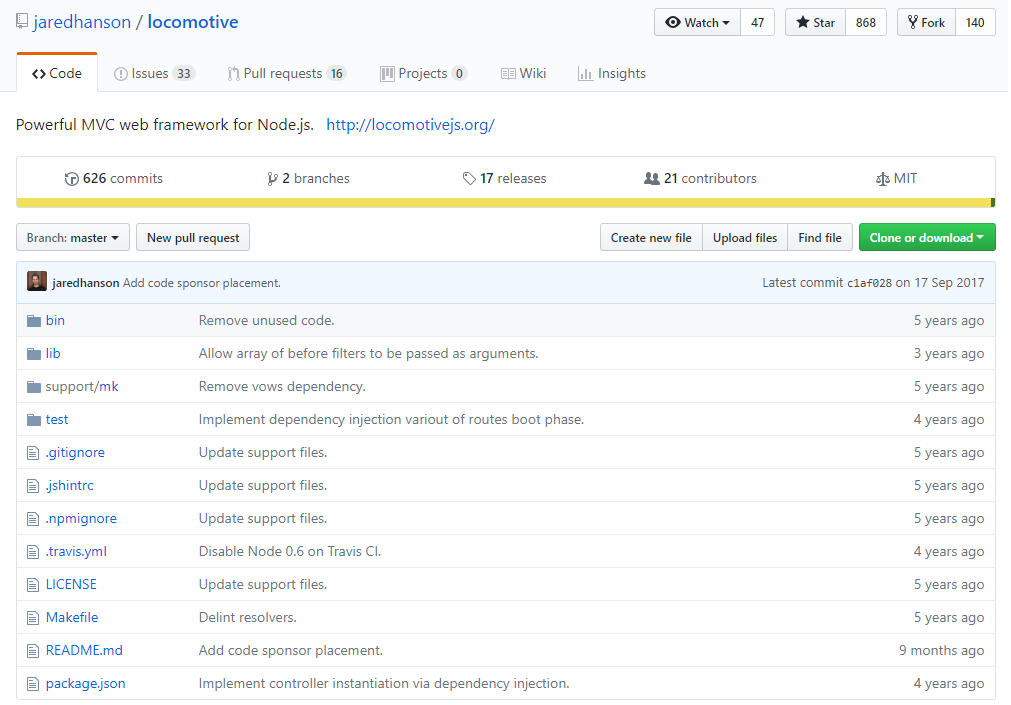
\includegraphics[width=\textwidth,height=\textheight,keepaspectratio]{locomotive.png} 
      \caption{Strona projektu locomotive w serwisie github, źródło: https://github.com/jaredhanson/locomotive/}
    \end{figure}
    Dla porównania framework koa posiada 21568 gwiazdek oraz był aktualizowany przed 9-cioma godzinami (dane na dzień 06.06.2018).
    Możemy wieć założyć że jest wciąż popularny oraz utrzymywany.
    \begin{figure}[!hb]
      \centering
      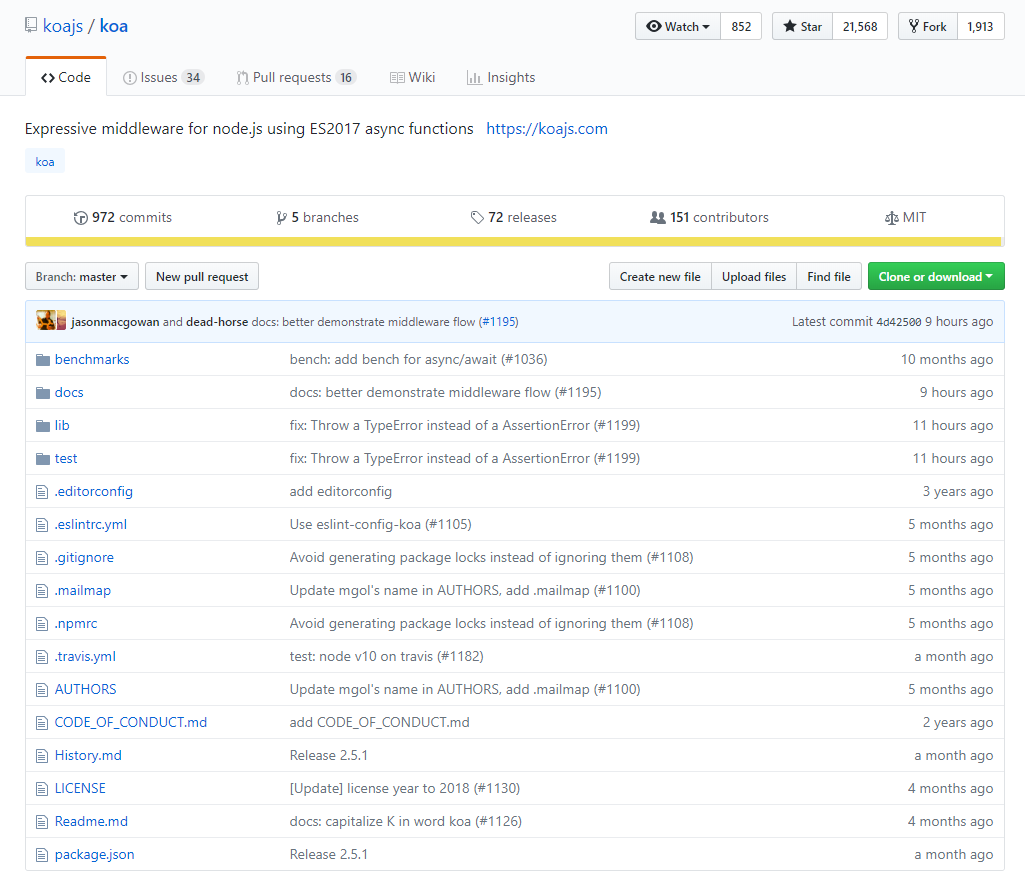
\includegraphics[width=\textwidth,height=\textheight,keepaspectratio]{koa.png} 
      \caption{Strona projektu koa w serwisie github, źródło: https://github.com/koajs/koa/}
    \end{figure}

  \section{Wybrane frameworki}
    Ilość dostępnych narzędzi nie pozwala niestety na porównanie wszystkich rozwiązań.
    W związku z czym zdecydowałem się przeanalizować w pracy 3 wybrane - express, sails oraz meteor.

    \subsection{Express}
      Express wybrałem ze wzgłedu na jego ogromną popularność.
      Repozytorium projektu posiada prawie 40000 gwiazdek w serwisie github oraz jest najpopularniejszy ze wszystkich frameworków w serwisie stackoverflow (dane na dzień 06.06.2018).
      Ze wszystkich konkurencyjnych rozwiązań jest najpopularniej wymienianą technologią w ofertach pracy.
      Został wybrany aby sprawdzić czy wiodące rozwiązanie jest słusznie liderem na rynku.
      \begin{figure}[!hb]
        \centering
        
\includegraphics[width=\textwidth,height=\textheight,keepaspectratio]{express.png} 
        \caption{Strona projektu express w serwisie github, źródło: https://github.com/expressjs/express}
      \end{figure}

    \subsection{Sails}
      Sails został wybrany ze wzgłędu na wyjątkowo niski próg wejścia.
      Framework dostarcza nam gotowy szkielet aplikacji, który musimy dostosować pod nasze wymagania.
      Nie zyskał on jeszcze tak dużej popularności jak pozostałe rozwiązania, jednak dzięki prostocie zbiera on coraz więcej fanów.
      Jego użytkownicy podkreślają skalowalność, szybkość oraz uzyskaną produktywność jako największe jego zalety.
      Repozytorium projektu posiada prawie 20000 gwiazdek w serwisie github (dane na dzień 06.06.2018).
      \begin{figure}[!hb]
        \centering
        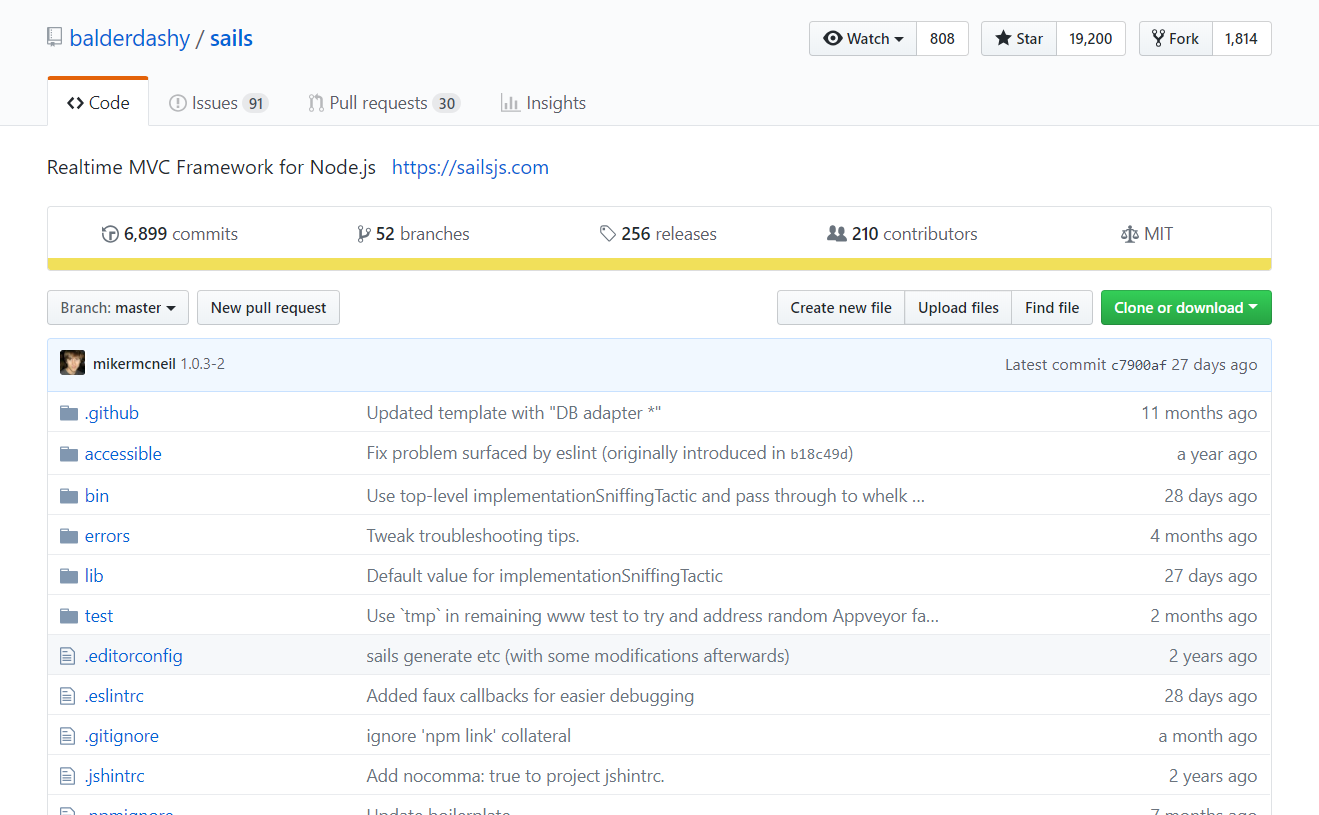
\includegraphics[width=\textwidth,height=\textheight,keepaspectratio]{sails.png} 
        \caption{Strona projektu sails w serwisie github, źródło: https://github.com/balderdashy/sails}
      \end{figure}

    \subsection{Meteor}
      Meteor wybrałem ponieważ mimo odcięcia się od tradycyjnego środowiska technologii Node.js, cieszy się on dużą popularnością oraz dostarcza nam możliwość wytwarzania jednocześnie częsci backendowej, frontendowej a nawet aplikacji mobilnych przy użyciu jednej bazy kodu.
      Framewok wprowadza wiele własnych narzędzi (np. własnego menadżera zależności, któremu w czystym Node.js odpowiada narzędzie npm) oraz gotowych modułów zarówno widoku jak i logiki pozwalając na efektywniejsze wytwarzanie gotowego produktu.
      Repozytorium projektu posiada blisko 40000 gwiadek w serwisie github (dane na dzień 06.06.2018).
      Popularność Meteora jest więc równa popularności frameworku express, mimo że jest on od niego 2 lata młodszy.
      \begin{figure}[!hb]
        \centering
        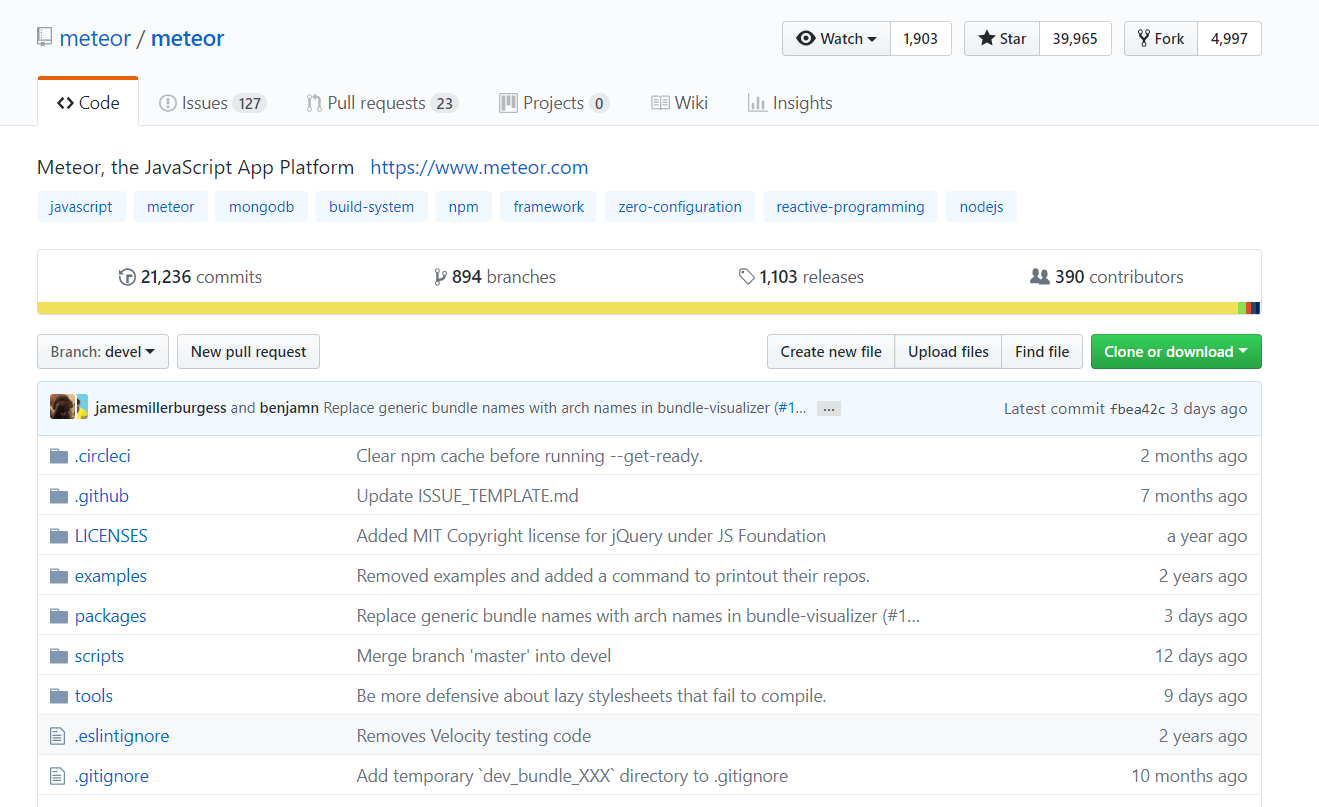
\includegraphics[width=\textwidth,height=\textheight,keepaspectratio]{meteor.png} 
        \caption{Strona projektu meteor w serwisie github, źródło: https://github.com/meteor/meteor}
      \end{figure}
  
  \section{Alternatywne rozwiązania}
    Alternatywne rozwiązania, które zostały wzięte pod uwagę to:

    \subsection{Hapi}
    Zaprojektowany do wytwarzania nowoczenych serwisów stron internetowych.
    Posiada wiele zdefiniowanych reużywalnych modułów (walidacja, cache, autentykacja) wymagających tylko minimalnej konfiguracji.
    Pozwala on na zminimalizowanie budowy infrastruktury projektu, na korzyść skupienia się na tworzeniu logiki oraz funkcjonalności.

    \subsection{Koa}
    Stworzony przez twórców frameworka express.
    Dostarcza możliwość wytwarzania częsci api serwisów.
    Po pierwszych prezentacjach Koa została przyjęta bardzo pozytywnie pozwalając na zminimalizowanie ilości pracy potrzebną na wytowrzenie produktu przy użyciu express'a.
    Narzędzie jest jednak ciągle w fazie silnego rozwoju i nie dostarcza jeszcze tak szerokich jak express możliwości.
    Z pewnością jest dla niego dobrą alternatywą w przypadku nieskomplikowanych serwisów.

    \subsection{Loopback}
    Framework fullstack'owy, zbudowany do tworzenia aplikacji mobilnych (ios, android) oraz aplikacji webowych wymagając bardzo niewielkich nakładów kodu.
    Do działania wykorzystuje express.
    Dzięki narzędzią takim jak IBM API Connect możemy wytwarząć kod przy użyciu graficznego interfejsu.

\chapter{Kryteria oceny}

  \section{Skala oraz wagi ocen}
    Rozdział opisuje jakie parametry frameworków zostały przeanalizowane i skonfrontowane ze sobą.
    Frameworki zostały ocenione w skali od 1 do 3 pod kątem każdego z nich.
    Każdy z parametrów otrzymał wagę w skali od 1 do 5.
    Wagi oznaczają wpływ danego parametru na ocene podsumowującą.
    Końcowe oceny zostały wyliczone ze wzoru:
    \newline
    \newline
    \[\text{\Large$O = \frac{\sum_{i=1}^{n} p_{i} * w_{i}}{n}$}\]
    gdzie:
    \begin{description}
      \item[O] - ocena końcowa
      \item[n] - ilość parametrów
      \item[p] - ocena parametru
      \item[w] - waga parametru
    \end{description}

  \section{Parametry}
    \subsection{Popularność}
      \begin{description}
        \item Waga: 3
      \end{description}
      Popularność jest wskaźnikiem, który niesie wiele infromacji na temat badanego frameworka.
      W najprostrzy sposób możemy ją sprawdzić za pomocą google trends, w przypadku narzedzi open source przy użyciu statystyk repozytorium, a w przypadku pozostałych poprzez serwisy stackoverflow.
      Dzięki popularności możemy wywnioskować wielokość społeczności jaka jest zainteresowana danym narzedziem.
      Wiąże się to z możliwym wsparciem, wartością rynkową oraz szerokością możliwych zastosowań jakie wspiera.
      Oczywistym jest że jeśli narzędzie posiada ogromną popularność zostało sprawdzone w dużej ilośći przypadków, a jeśli potrafi im sprostać umiejętności sprawnego posługiwania się nim stają się cenniejsze.
      \subsection{Rozmiar frameworku}
      \begin{description}
        \item Waga: 1
      \end{description}
      Rozmiar frameworku ma bezpośredni wpływa na rozmiar naszego końcowego produktu.
      Najbardziej pożądane jest aby narzędzie zajmowało jak najmniej miejsca.
      W celu zminimalizowania rozmiaru naszego produktu możemy użyć bundlerów takich jak np. weback, które sprawią że do końcowego produktu zostanie załączona wyłącznie taka funkcjonalność biblioteki którą rzeczywiście wykorzystujemy.
      Warto o tym pamiętać w przypadku użycia dużych narzędzi dla prostych, niewymagających rozwiązań.
      Mimo takowej możliwości nie gwarantuje nam to zawsze małego rozmiaru produktu, dlatego rozmiar frameworku został wzięty pod uwagę.

    \subsection{Dokumentacja}
      \begin{description}
        \item Waga: 3
      \end{description}
      Nawet najbardziej użyteczne narzędzie nie mogłoby zaistnieć bez łatwo dostępnej, zrozumiale przekazanej dokumentacji.
      Jest ona niezbędna do przyswojenia proponowanych konceptów oraz obycia się z wybranym rozwiązaniem.
      Ocena dokumentacji dotyczy jej dostępności, szczegółowości oraz zrozumiałości.

    \subsection{Próg wejścia}
      \begin{description}
        \item Waga: 1
      \end{description}
      Próg wejścia oznacza ilość zagadnień wymaganych w celu opanowania danego frameworka oraz ilość czasu jaki należy poświęcić na jego opanowanie w stopniu conajmniej podstawowym.
      Pożądane jest aby był on jak najniższy; aby narzędzie nadawało się do użycia przez osoby jak najsłabiej znające koncepty programowania czy budowy systemów, niemal że natychmiast po chwilowym zapoznaniu się z dokumentacja.

    \subsection{Warstwa widoku}
      \begin{description}
        \item Waga: 2
      \end{description}
      Parametr opisuje w jakim stopniu badany framework zapewnia obsluge warstwy widoku wytwarzanej aplikacji.
      Możemy oczekiwać wielu możliwości obsługi warstwy widoku.
      Wydawać by się mogło, że dla najlepszą możliwością byłoby gdyby framework kompletnie integrował warstwe widoku z warstwą danych dostarczając określone, proste metody wzajemnego mapowania.
      Kompletnie nie porządane jest aby do obsługi oraz integracji z warstwą widoku wytwarzanego produktu było wymagane użycie zewnętrznego, dodatkowego narzędzia.

    \subsection{Warstwa bazy danych}
      \begin{description}
        \item Waga: 2
      \end{description}
      Podobnie jak parametr warstwy widoku, parametr ten opisuje możliwość integracji frameworka z bazą danych.
      Najmniej pożądanym zachowaniem jest kiedy moduł obsługi bazy danych należy w całości dołączyć do rozwiązania, natomiast najbardziej pożądanym aby framework w pełni posiadał zaimplementowaną integracje przy użyciu np komponentu DAO.

    \subsection{Szybkość przetwarzania zapytań}
      \begin{description}
        \item Waga: 3
      \end{description}
      Parametr opisuje ilość przetworzonych zapytań w ciągu określonego czasu.
      Kolejne zapytania zostają wysłane dopiero po otrzymaniu odpowiedzi na poprzednie.
      Możemy w ten sposób sprawdzić jak sprawnie aplikacja wykonana w konkretnym środowisku jest w stanie odpowiadać na nieustające zapytania końcowego użytkownika.
      Zapytania zostały dobranego dla różnych przypadków użycia:
      \begin{description}
        \item Autoryzacja - uzyskanie autoryzacji na zapytanie zawierające login oraz hasło użytkownika
        \item Zapis danych użytkownika - zapisanie podstawowych danych użytkownika w bazie danych
        \item Proste zapytanie o zasób - uzyskanie dostępu do zasobu tekstowego z bazy danych przez użytkownika
        \item Zapytanie o zasób - uzyskanie dostępu do zasobu multimedialnego (pliku w formacie jpg) z serwera
        \item Streaming multimediów - uzyskanie dostępu do streamu multimedialnego (w formacie avi) z serwera
      \end{description}
      Okresy czasu dla których zostały wykonane testy to:
      \begin{description}
        \item krótki - 1 sekunda
        \item średni - 15 sekunda
        \item długi - 60 sekund
      \end{description}
      
    \subsection{Szybkość przetwarzania zapytań równoległych}
      \begin{description}
        \item Waga: 3
      \end{description}
      Parametr opisuje czas potrzebny na przetworzenie różnych ilości równolegle przychodzących zapytań, symulując prace serwera przy obciążeniu od wielu użytkowników w tym samym czasie.
      Zapytania zostały wysłane w tym samym momencie i został zmierzony czas po którym uzyskano odpowiedź na wszystkie z nich.
      Zapytania zostały dobrane dla następujących przypadków użycia:
      \begin{description}
        \item Autoryzacja - uzyskanie autoryzacji na zapytanie zawierające login oraz hasło użytkownika
        \item Zapis danych użytkownika - zapisanie podstawowych danych użytkownika w bazie danych
        \item Proste zapytanie o zasób - uzyskanie dostępu do zasobu tekstowego z bazy danych przez użytkownika
        \item Zapytanie o zasób - uzyskanie dostępu do zasobu multimedialnego (pliku w formacie jpg) z serwera
        \item Streaming multimediów - uzyskanie dostępu do streamu multimedialnego (w formacie avi) z serwera
      \end{description}
      Ilości wysłanych równolegle zapytań to:
      \begin{description}
        \item mała - 20 zapytań
        \item średnia - 200 zapytań
        \item duża - 2000 zapytań
      \end{description}

    \subsection{Ilość kodu do napisania}
      \begin{description}
        \item Waga: 2
      \end{description}
      Parametr opisuje ilość kodu potrzebnego do napisania aby otrzymać taką samą funkcjonalność w analizowanych środowiskach.
      Ilość kodu pisanego przy użyciu tego samego języka oraz jego standardu z zachowaniem odpowiednich praktych może zostać przełożony na ilość pracy, a co za tym idzie czasu jaką należy poświęcić do osiągnięcia obranego celu.
      Stworzony kod musi dotyczyć zarówno części frontendowej jak i backendowej.
      Do analizy została wybrana zadana funkcjonalność:
      \begin{description}
        \item Autoryzacja - uzyskanie autoryzacji na zapytanie zawierające login oraz hasło użytkownika
        \item Zapis danych użytkownika - zapisanie podstawowych danych użytkownika w bazie danych
        \item Proste zapytanie o zasób - uzyskanie dostępu do zasobu tekstowego z bazy danych przez zautoryzowanego użytkownika
        \item Zapytanie o zasób - uzyskanie dostępu do zasobu multimedialnego (pliku w formacie jpg) z serwera
        \item Streaming multimediów - uzyskanie dostępu do streamu multimedialnego (w formacie avi) z serwera
      \end{description}
      Napisany kod musi być zgodny ze stosowanymi, ogólnie uznanymi praktykami programistycznymi dla danych środowisk.

    \subsection{Rozszerzalność}
      \begin{description}
        \item Waga: 3
      \end{description}

    \subsection{Testowanie}
      \begin{description}
        \item Waga: 2
      \end{description}

\chapter{Opis wybranych rozwiązań}

  \section{ExpressJS}
  \section{Sails}
  \section{Meteor}

\chapter{Analiza porównawcza}

  \section{ExpressJS}
    \subsection{Rozmiar frameworku}
    \subsection{Popularność}
    \subsection{Dokumentacja}
    \subsection{Próg wejścia}
    \subsection{Warstwa widoku}
    \subsection{Warstwa bazy danych}
    \subsection{Szybkość przetwarzania zapytań}
    \subsection{Szybkość przetwarzania zapytań równoległych}
    \subsection{Ilość kodu do napisania}
    \subsection{Rozszerzalność}
    \subsection{Testowanie}

  \section{Sails}
    \subsection{Rozmiar frameworku}
    \subsection{Popularność}
    \subsection{Dokumentacja}
    \subsection{Próg wejścia}
    \subsection{Warstwa widoku}
    \subsection{Warstwa bazy danych}
    \subsection{Szybkość przetwarzania zapytań}
    \subsection{Szybkość przetwarzania zapytań równoległych}
    \subsection{Ilość kodu do napisania}
    \subsection{Rozszerzalność}
    \subsection{Testowanie}

  \section{Meteor}
    \subsection{Rozmiar frameworku}
    \subsection{Popularność}
    \subsection{Dokumentacja}
    \subsection{Próg wejścia}
    \subsection{Warstwa widoku}
    \subsection{Warstwa bazy danych}
    \subsection{Szybkość przetwarzania zapytań}
    \subsection{Szybkość przetwarzania zapytań równoległych}
    \subsection{Ilość kodu do napisania}
    \subsection{Rozszerzalność}
    \subsection{Testowanie}

\chapter{Podsumowanie}
  \section{Podsumowanie ocen}
  \section{Wskazywane zastosowania}

\addcontentsline{toc}{chapter}{Bibliografia}

\begin{thebibliography}{99}
  \bibitem{Brown}
    E. Brown
    \textit{"Web Development with Node and Express", 2014}

  \bibitem{Mardan}
    Azat Mardan
    \textit{"Express.js Guide: The Comprehensive Book on Express.js", 2016}

  \bibitem{StrongLoop}
    StrongLoop
    \textit{dokumentacja Express, 2017, źródło: https://expressjs.com/en/4x/api.html}

  \bibitem{McNeil&Nathan}
    Mike McNeil, Irl Natha
    \textit{"Sails.js in Action", 2017}

  \bibitem{Shahid}
    Shahid Shaikh
    \textit{"Sails.js Essentials", 2016}

  \bibitem{McNeil}
    Mike McNeil
    \textit{dokumentacja Sails, 2017, źródło: https://sailsjs.com/documentation/reference}

  \bibitem{Strack}
    Isaac Strack
    \textit{"Getting Started with Meteor JavaScript Framework", 2012}

  \bibitem{Vogelsteller&Strack&Reyna}
    Fabian Vogelsteller, Isaac Strack, Marcelo Reyna
    \textit{"Meteor: Full-Stack Web Application Development", 2016}

  \bibitem{MDG}
    Meteor Development Group
    \textit{dokumentacja Meteor API, 2017, źródło: https://docs.meteor.com/\#/full/}

  \bibitem{Onodi}
    Node.js Foundation
    \textit{dokumentacja języka programowania Node.js, 2017, źródło: https://nodejs.org/en/docs/}

  \bibitem{Wolff}
    Eberhard Wolff
    \textit{"Microservices: Flexible Software Architecture", 2016}

  \bibitem{Zeidman}
    Bob Zeidman
    \textit{"The Software IP Detective's Handbook: Measurement, Comparison, and Infringement Detection", rok}

\end{thebibliography}

\addcontentsline{toc}{chapter}{Spis rysunków}

\listoffigures

\end{document}